\documentclass[tikz,border=10pt]{standalone}
\usepackage{amsmath}
\usepackage{amssymb}
\begin{document}

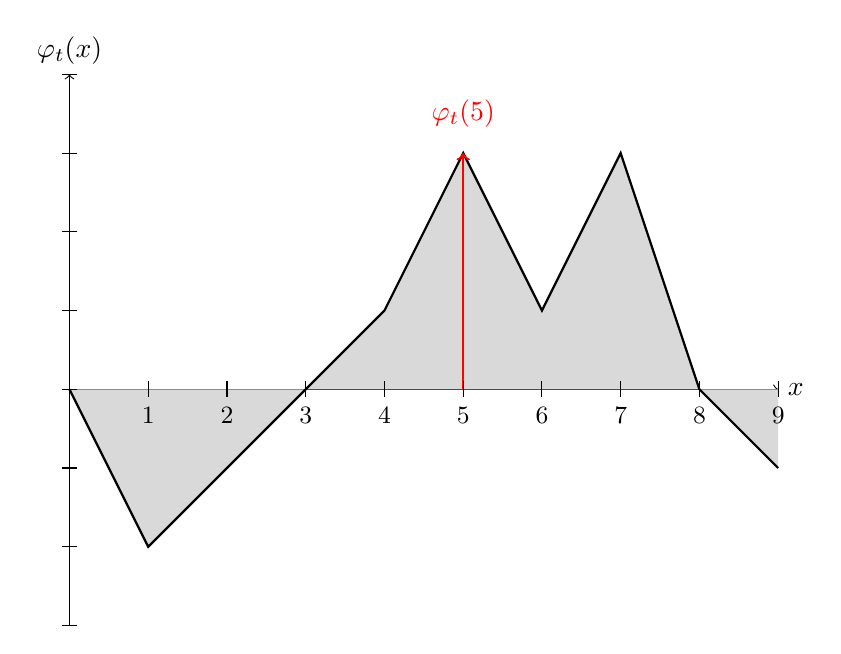
\begin{tikzpicture}

% Axes
\draw[->] (0,0) -- (9,0) node[right] {$x$};
\draw[->] (0,-3) -- (0,4) node[above] {$\varphi_t(x)$};

% Fluctuating interface
\fill[gray!30] (0,0) -- (1,-2) -- (2,-1) -- (3,0) -- (4,1) -- (5,3) -- (6,1) -- (7,3) -- (8,0) -- (9,-1) -- (9,0) -- cycle;

% Interface line
\draw[thick] (0,0) -- (1,-2) -- (2,-1) -- (3,0) -- (4,1) -- (5,3) -- (6,1) -- (7,3) -- (8,0) -- (9,-1);

% Highlighted line at x=5
\draw[red, thick, ->] (5,0) -- (5,3);

% Labels
\node at (5,3.2) [above, red] {$\varphi_t(5)$};

% x-axis ticks
\foreach \x in {1,...,9}
  \draw (\x,0.1) -- (\x,-0.1) node[below] {\small $\x$};

% y-axis ticks
\foreach \y in {-3,-2,...,4}
  \draw (0.1,\y) -- (-0.1,\y);

\end{tikzpicture}

\end{document}